\chapter{深度学习基础}
深度学习概括介绍...

本章主要介绍深度学习的理论基础,包括感知器、激活函数、反向传播算法、卷积神经网络等相关概念与理论。
\section{感知器}
感知器(perceptron)是构成神经网络的基础,感知器的概念由 Frank Rosenblatt 在 1950 年代到 1960 年代基于 Warren McCulloch 和 
Walter Pitts 的关于人类神经活动的模拟的研究提出并发展而来。如今最常用的感知器被称作 sigmoid 感知器,但是它的基础仍然是最初提出的感知器模型,
下面对其原理进行介绍。

\begin{figure}[h]
	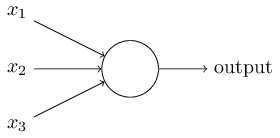
\includegraphics{perceptron.png}
	\caption{感知器模型}
	\label{perceptron}
\end{figure}

如图//所示,感知器接收若干个二进制输入$x_1, x_2, x_3, ...$并输出一个二进制结果。Rosenblatt 提出了一种计算感知机输出值的简易准则,他引入“权重(weight)”
的概念,用实数$w_1, w_2,...$来表示每个输入的重要性。最后神经元的输出,0 或者 1,是由加权和 $\sum_j w_{j}x_{j}$是否小于某个门限值决定的。和
权重一样,门限值也是神经元的一个实数参数。以上准则可由下面的公式\ref{eqn:perceptron}表示:
\begin{equation}
\label{eqn:perceptron}
output = \left\{ \begin{array} { l l } { 0 } & { \text { if } \sum _ { j } w _ { j } x _ { j } \leq \text { 门限 } } \\ { 1 } & { \text { if } \sum _ { j } w _ { j } x _ { j } > \text { 门限 } } \end{array} \right.
\end{equation}

以上就是感知器的简单数学模型。可以把感知器看成是一种对输入特征进行加权并输出决策的设备。可以结合实际举一个简单的例子。假如某人要决定周末是否
外出游玩,那么影响他决策的因素就可能是以下三个方面:

1. 天气是否晴好?

2. 是否有同伴陪同?

3. 游玩地点是否在地铁站附近?

我们可以用变量$x_1, x_2, x_3$来表征这三个二进制影响因素,比如$x_1 = 1$表示天气晴好,$x_2 = 1$表示有同伴陪同,$x_3 = 1$表示目标地点在地铁站
附近。

以上三个影响因素对最后的决定的影响程度是不一样的,这就需要对每个影响因素设置一个权重。假如天气是最关键的决定因素,在天气坏的情况下仍然出门的可能性很小,
那么就可将$x_1$对应的权重设置为$w_1=6$,其余两个影响因素的权重都设置为$w_2=1, w_3=1$。现在假如我们把门限值设置为 3,那么在天气坏的情况下,无论
其他两个因素是什么样的,最后的加权和都不会超过 3,从而做出周末不外出游玩这个决定。

通过设置不同的权重和门限,可得到不同的决策模型。比如将门限值降低可增加外出游玩的可能性,将是否有同伴陪同的权重提高可增加同伴对外出游玩与否的影响程度。

显然以上的感知器模型并不能完全体现人类决策的复杂性而只是一个简单的示例。通过堆叠多层感知器,可得到做出更加微妙决策的感知器网络:

\begin{figure}[h]
	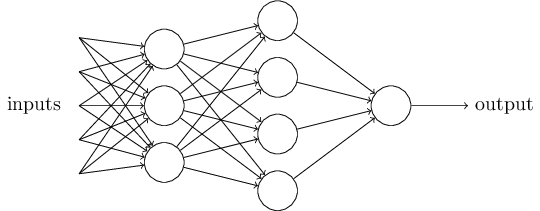
\includegraphics{layeredperceptron.png}
	\caption{多层感知器模型}
	\label{layeredperceptron}
\end{figure}

如图xx,第一层感知器一共做出三项简单决策,这三项决策又接着输入到第二层的四个感知器得出四个更进一步的决策,最后这四个决策又输入到最后一个感知器得到
最后的决策。这种级联方式可以让后面的感知器得出比前面的感知器更抽象的结果,从而解决更加复杂的决策问题。

通过引入“偏置(bias)”$b$,公式\ref{eqn:perceptron}也可以改写为公式\ref{eqn:perceptronbias}:
\begin{equation}
	\label{eqn:perceptronbias}
output = \left\{ \begin{array} { l l } { 0 } & { \text { if } w \cdot x + b \leq 0 } \\ { 1 } & { \text { if } w \cdot x + b > 0 } \end{array} \right.
\end{equation}

偏置的概念可理解为输出 1 的容易程度。从生物学的角度也可说成神经元达到激发态的容易程度。偏置的引入可简化后面的公式表示。

\section{激活函数}
本节所介绍的 sigmoid 激活函数的引入是为了使人工神经网络中感知器的权重和偏置的自动化训练成为可能。如果我们想通过调整感知器参数从而使网络的整体
表现满足某种特定需求,那么对感知器参数的微小改动必须也对应输出的微小改动,即稍稍改变权重和偏置不会导致输出的剧烈变化。前面的感知器模型只能输出0和1
两种结果,显然不能满足输出缓慢变化的特征。为了得到满足这种特征的感知器,需要对上节感知器模型做出修改,在输出时应用 sigmoid 函数$\sigma$:
\begin{equation}
	\label{eqn:sigmoid}
	\sigma ( z ) \equiv \frac { 1 } { 1 + e ^ { - z } }
\end{equation}

即,对于输入$x_1, x_2, ...$,权重$w_1, w_2, w_3,...$ 和权重 $b$,sigmoid 神经元的输出是:
\begin{equation}
	\label{eqn:sigmoidoutput}
	\frac { 1 } { 1 + \exp \left( - \sum _ { j } w _ { j } x _ { j } - b \right) }
\end{equation}
从图xx可以看出,本质上 sigmoid 函数是阶跃函数的平滑版本,这也说明了为什么 sigmoid 激活函数的引入可以解决输出剧烈变化的问题。

//sigmoid 阶跃函数对比

$\sigma$ 函数的重要性在于其平滑性,而与其具体的形状并没有太大的关系,$\sigma$ 的平滑度意味着权重中的微小变化
$\Delta w_j$ 和偏置中的 $\Delta w_j$ 将在神经元的输出中产生小的变化 $\Delta output$。
 事实上,微积分告诉我们 $\Delta output$ 很接近:
\begin{equation}
	\label{eqn:sigmoiddelta}
	\Delta \mathrm { output } \approx \sum _ { j } \frac { \partial \mathrm { output } } { \partial w _ { j } } \Delta w _ { j } + \frac { \partial \text { output } } { \partial b } \Delta b
\end{equation}

$\sigma$ 函数并不是唯一的激活函数形式,常用的激活函数还有 ReLU 激活函数。此函数是一个分段线性函数:
\begin{equation}
	\label{eqn:relu}
	\operatorname { ReLU } ( x ) = \left\{ \begin{array} { l l } { x } & { \text { if } x > 0 } \\ { 0 } & { \text { if } x \leq 0 } \end{array} \right.
\end{equation}

函数图像是:

//图:relu曲线图

从公式和图可以观察到 ReLU 函数把所有的负值都变为0,而正值线性变化,这种操作叫做单侧抑制。
尤其体现在深度神经网络模型(如CNN)中,当模型增加N层之后,理论上 ReLU 神经元的激活率将降低2的N次方倍。
相对于 sigmoid 函数,ReLU 能更好地实现网络模型的稀疏性,同时也符合近年来神经科学对神经元工作稀疏性的研究【引用】,同时 ReLu 在
正区间梯度总是为定值的特性也有利于避免梯度消失问题。

\section{神经网络结构}


\subsection{空间基函数}
RWG 基函数是定义在三角形单元上的最具代表性的基函数。它的具体定义如
下:
\begin{equation}
f_n(r)=
\begin{cases}
\frac{l_n}{2A_n^+}\rho_n^+=\frac{l_n}{2A_n^+}(r-r_+)&r\in T_n^+\\
\frac{l_n}{2A_n^-}\rho_n^-=\frac{l_n}{2A_n^-}(r_--r)&r\in T_n^-\\
0&\text{otherwise}
\end{cases}
\end{equation}

其中,$l_n$为三角形单元$T_n^+$和$T_n^-$公共边的长度,$A_n^+$和$A_n^-$分别为三角形单元$T_n^+$和$T_n^-$的面积(如图\ref{pica}所示)。

\begin{figure}[h]
	\includegraphics{pica.pdf}
	\caption{RWG 基函数几何参数示意图}
	\label{pica}
\end{figure}
由于时域混合场积分方程是时域电场积分方程与时域磁场积分方程的线性组合,因此时域混合场积分方程时间步进算法的阻抗矩阵特征与时域电场积分方程时间步进算法的阻抗矩阵特征相同。
\begin{equation}
\label{latent_binary_variable}
\mathbf{r}_{i,j}=
\begin{cases}
1,f(\mathbf{x}^{i};\mathbf{w})\cdot f(\mathbf{x}^{j};\mathbf{w})\geq u(\lambda),\\
0,f(\mathbf{x}^{i};\mathbf{w})\cdot f(\mathbf{x}^{j};\mathbf{w})< l(\lambda), 1\leq i,j\leq n.\\
f(\mathbf{x}^{i};\mathbf{w})\cdot f(\mathbf{x}^{j};\mathbf{w}),\text{otherwise},
\end{cases}
\end{equation}

时域积分方程时间步进算法的阻抗元素直接影响算法的后时稳定性,因此阻抗元素的计算是算法的关键之一,采用精度高效的方法计算时域阻抗元素是时域积分方程时间步进算法研究的重点之一。


\subsection{时间基函数}

\subsubsection{时域方法特有的展开函数}

\subsubsection{频域方法特有的展开函数}

\section{入射波}

如图\ref{picb}和图\ref{picc}所示分别给出了参数$E_0=\hat{x}$,$a_n=-\hat{z}$,$f_0=250MHz$,$f_w=50MHz$,$t_w=4.2\sigma$时,调制高斯脉冲的时域与频域归一化波形图。

\begin{figure}[h]
	\subfigure[]{
		\label{picb}
		\includegraphics[width=7.3cm]{picb.pdf}}
	\subfigure[]{
		\label{picc}
		\includegraphics[width=6.41cm]{picc.pdf}}
	\caption{调制高斯脉冲时域与频率波形,时域阻抗元素的存储技术也是时间步进算法并行化的关键技术之一,采用合适的阻抗元素存储方式可以很大的提高并行时间步进算法的计算效率。}
	\label{fig1}
\end{figure}
时域阻抗元素的存储技术\citing{xiao2012yi}也是时间步进算法并行化的关键技术之一,采用合适的阻抗元素存储方式可以很大的提高并行时间步进算法的计算效率。

\section{本章小结}
本章首先从时域麦克斯韦方程组出发推导得到了时域电场、磁场以及混合场积分方程。

\chapter{时域积分方程数值方法研究}
\section{时域积分方程时间步进算法的阻抗元素精确计算}
时域积分方程时间步进算法的阻抗元素直接影响算法的后时稳定性,因此阻抗元素的计算是算法的关键之一,采用精度高效的方法计算时域阻抗元素是时域积分方程时间步进算法研究的重点之一。

\section{时域积分方程时间步进算法阻抗矩阵的存储}
时域阻抗元素的存储技术也是时间步进算法并行化的关键技术之一,采用合适的阻抗元素存储方式可以很大的提高并行时间步进算法的计算效率。

\subsection{时域积分方程时间步进算法产生的阻抗矩阵的特征}
由于时域混合场积分方程是时域电场积分方程与时域磁场积分方程的线性组合,因此时域混合场积分方程时间步进算法的阻抗矩阵特征与时域电场积分方程时间步进算法的阻抗矩阵特征相同。

\subsection{数值算例与分析}

如图3-1(a)所示给出了时间步长选取为0.5ns时采用三种不同存储方式计算的平板中心处 方向的感应电流值与IDFT方法计算结果的比较。如图3-1(b)所示给出了存储方式为基权函数压缩存储方式,时间步长分别取时平板中心处 方向的感应电流计算结果,从图中可以看出不同时间步长的计算结果基本相同。

\begin{algorithm}[H]
	\KwData{this text}
	\KwResult{how to write algorithm with \LaTeX2e }
	initialization\;
	\While{not at end of this document}{
		read current\;
		\eIf{understand}{
			go to next section\;
			current section becomes this one\;
		}{
		go back to the beginning of current section\;
	}
}
\caption{How to wirte an algorithm.}
\end{algorithm}

由于时域混合场积分方程是时域电场积分方程与时域磁场积分方程的线性组合,因此时域混合场积分方程时间步进算法的阻抗矩阵特征与时域电场积分方程时间步进算法的阻抗矩阵特征相同。

\section{时域积分方程时间步进算法矩阵方程的求解}

\section{本章小结}
本章首先研究了时域积分方程时间步进算法的阻抗元素精确计算技术,分别采用DUFFY变换法与卷积积分精度计算法计算时域阻抗元素,通过算例验证了计算方法的高精度。
